\chapter{METHODOLOGY}
\label{ch:methodology}

% This is Chapter 3 - Methodology
% Describe your research methodology and approach

\section{Introduction}

This chapter describes in detail the methodology used to conduct a controller comparison of the three lightest variants of the YOLOv8 model: nano (YOLOv8n), small (YOLOv8s), and medium (YOLOv8m). The specific task under which they will be tested is the detection of the four distinct classes of player, referee, goalkeeper and ball. The evaluation consists of two primary dimensions, detection accuracy and inference speed. The environment under which the models will be tested consists of three consumer level hardware configurations, in order to offer a real picture of what a low budget practitioner will experience when using them.

\section{Research Design}

The target variable of this study is the moder architecture and scale. As such, measures have to be taken in order to not allow any other factors to influence the results. The three YOLOv8 variants share identical architectural topology and differ only in depth and width scaling coefficients, which in turn determine parameter count and computational cost. This property makes them perfect for a comparative study such as this one, as any differences that get observed would be as an unambiguous result of model capacity and not due to architecture, training pipeline, or data processing.

To give each model the same conditions, all other influencing attributes have to remain identical. This includes the dataset, the way it is preprocessed, training hyperparameters, augmentation configuration and the inference settings during evaluation. Training is conducted once on a single machine equipped with a dedicated GPU. It follows a fine-tuning approach which starts from COCO pretrained weights then learns the domain-related details from our dataset. Inference benchmarking is conducted on each of the three devices using the same trained weights and test video. From this we can conclude that all latency differences will be purely as a result of the interaction between model and hardware.


\section{Dataset}

\subsection{Source}

The dataset used in this study is the Bundesliga Data Shootout dataset, published by Delfos (2022)\cite{RN18} and hosted on the Roboflow Universe platform. It was downloaded via the Roboflow Python API, ensuring reproducibility across machines. The dataset consists of annotated frames extracted from broadcast footage of Bundesliga football matches, making it particularly relevant to the detection task this thesis studies. It was selected because it provides YOLO-format annotations compatible with the Ultralytics pipeline, covers all four object classes of interest (players, goalkeepers, referees, and the ball), and is publicly versioned, enabling easy future replication. For our testing, however, we trained our models on the two most relevant classes, the player and ball class, in order to get the most direct result on what coaches and scouts might need when evaluating talent.

\subsection{Dataset Splitting}
The dataset version downloaded from Roboflow includes a predefined train, validation, and test split. Using the predefined split, rather than applying a random split at training time, serves two purposes. First, it ensures that the same images appear in the same partitions across all three models, so that accuracy differences cannot be attributed to variation in which images each model saw during training. Second, it enables direct comparison with future studies that use the same dataset version, as the evaluation set is fixed and consistent.

\subsection{Data Augmentation}
Augmentation for this study was applied in two distinct stages: offline augmentation performed by Roboflow at dataset export time, and online augmentation applied by the YOLOv8 training pipeline during each epoch. Understanding both stages is necessary for an accurate account of the data the models were trained on. 

The Roboflow export configuration applied the following augmentations to the base dataset, generating three augmented outputs per original training image and thereby tripling the effective training set size: horizontal and vertical flipping, clockwise and counterclockwise 90° rotations, rotation between -15° and +15°, hue jitter between -20° and +20°, saturation jitter between -25\% and +25\%, exposure jitter between -10\% and +10°, and Mosaic compositing. Several of these augmentations are well-suited to broadcast football footage. Horizontal flipping is appropriate given the bilateral symmetry of the pitch. HSV-space jitter addresses variation in broadcast lighting conditions and camera white balance. Mosaic augmentation, which composites four images into a single training sample, is particularly beneficial for small-object detection and increases the frequency with which the ball appears at varied scales and positions within a single training image.

\begin{figure}[h]
    \centering
    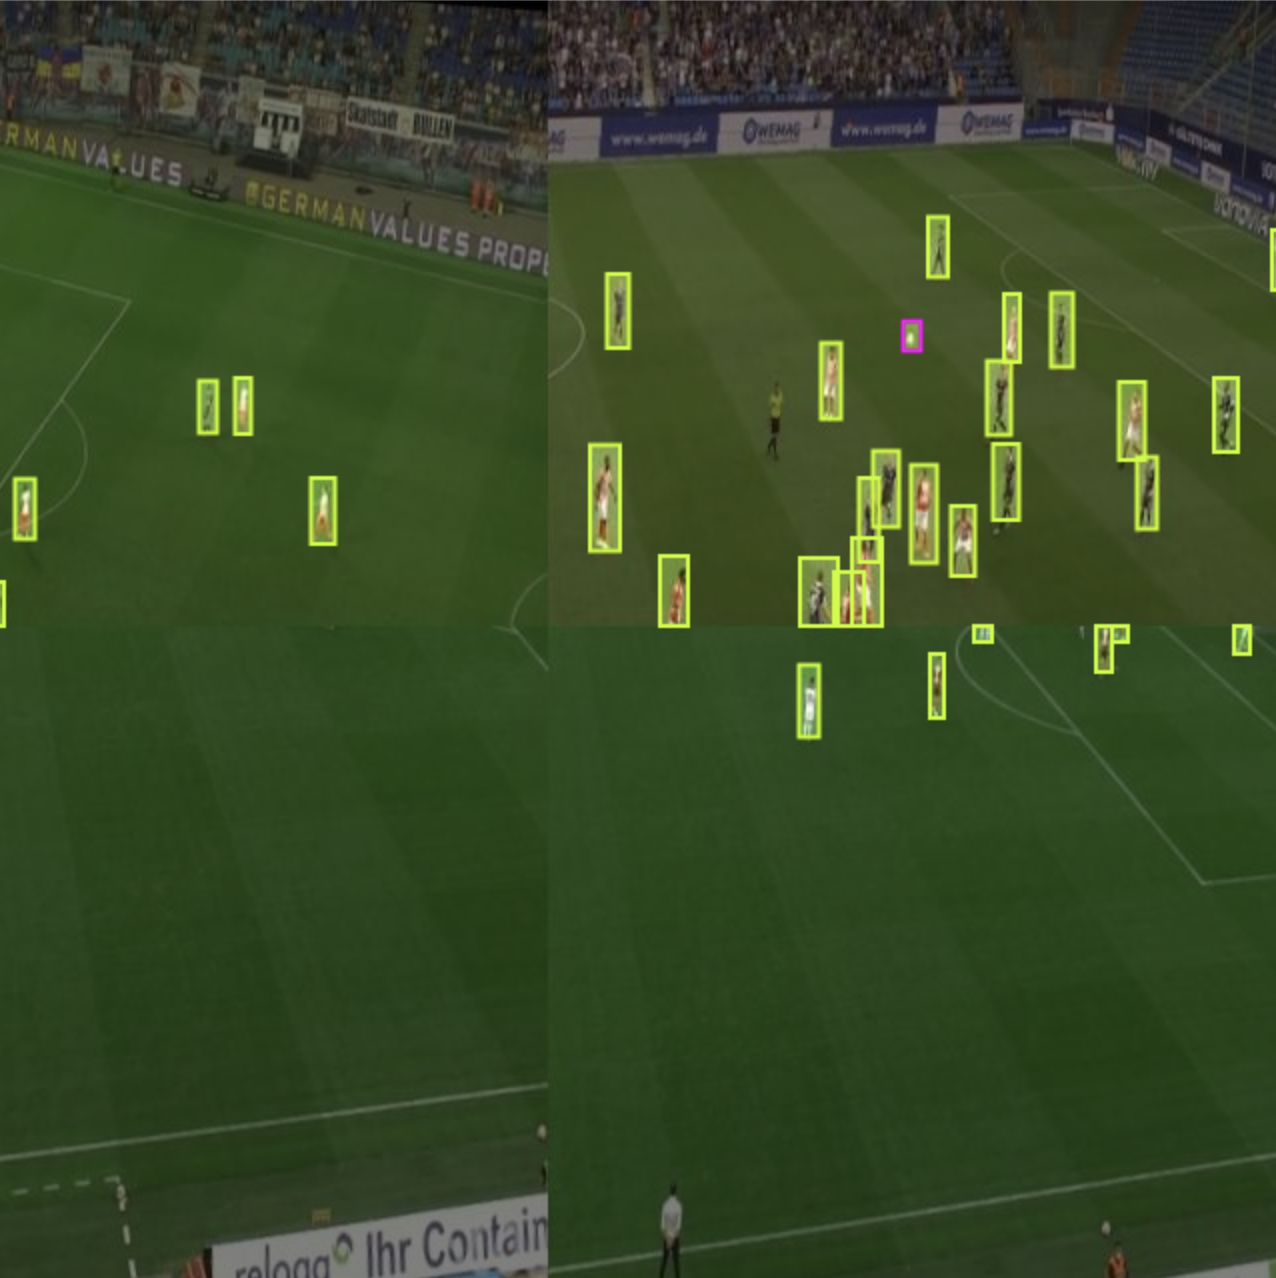
\includegraphics[width=0.8\textwidth]{figures/dataset example.png}
    \caption{An example of an annotated and augmented image in our dataset\cite{RN18}}
    \label{fig:image_example}
\end{figure}

The augmentations are not perfect, however, and make up some of the limitations of this study. Vertical flipping and 90° rotations produce frames that are sure to never show up on regular usage input, as football broadcast footage is always oriented horizontally relative to the pitch. 

The online augmentation performed applied by the YOLO training pipeline has been left at default. The reasoning for this is that the aim of this study is not to create the absolute best model, rather to focus more on the accuracy-speed balance on different hardware configurations. 

\begin{table}[h]
\centering
\label{tab:roboflow_augmentation}
\begin{tabular}{ll}
\hline
\textbf{Augmentation} & \textbf{Setting} \\
\hline
Horizontal flip          & Applied  \\
Vertical flip            & Applied  \\
90\textdegree{} rotation (CW and CCW) & Applied  \\
Rotation                 & $\pm$15\textdegree{}  \\
Hue jitter               & $\pm$20\textdegree{}  \\
Saturation jitter        & $\pm$25\%  \\
Exposure jitter          & $\pm$10\%  \\
Mosaic                   & Applied  \\
Outputs per image        & 3$\times$  \\
\hline
\end{tabular}
\caption{Augmentation configuration applied to the dataset from default Roboflow configurations.}
\end{table}



\section{Training Procedure}

Due to the relatively small size of our dataset, a transfer learning strategy is implemented with the goal to avoid high variance results. The COCO dataset offers low-level visual features which are shared with broadcast footage. This in turn allows the model to rapidly adapt to class distributions specific to our domain. 

The key requirement for a valid comparative evaluation is that all hyperparamaters remain equal for all model variants. To achieve this, a single configuration dictionary is defined and shared to all models in their training call. The full configuration is described in table 3.2.

\begin{table}[h]
\centering

\label{tab:training_config}
\begin{tabular}{lp{2cm}p{7cm}}
\hline
\textbf{Parameter} & \textbf{Value} & \textbf{Justification} \\
\hline
\texttt{epochs}        & 50      & Sufficient for convergence; early stopping prevents overfitting \\ \hline
\texttt{imgsz}         & 640     & YOLOv8 standard input resolution \\ \hline
\texttt{optimizer}     & SGD     & Default YOLOv8 optimizer; identical dynamics across variants \\ \hline
\texttt{lr0}           & 0.01    & Default YOLOv8 learning rate; explicitly locked \\ \hline
\texttt{nbs}           & 64      & Nominal batch size; ensures identical effective LR scaling across variants \\ \hline
\texttt{batch}         & 8       & Physical batch size fitting RTX 3060 12\,GB VRAM for all variants \\ \hline
\texttt{amp}           & False   & Full FP32; prevents hardware-specific numeric differences \\ \hline
\texttt{seed}          & 42      & Fixed seed for reproducible weight initialization and data ordering \\ \hline
\texttt{deterministic} & True    & Disables non-deterministic CUDA ops for reproducibility \\ \hline
\texttt{patience}      & 20      & Proportionate to 50-epoch budget; allows recovery from plateaus \\ \hline
\end{tabular}
\caption{Shared training configuration applied identically to all three YOLOv8 variants.}
\end{table}

A physical batch size of 8 is used for all three variants to fit within the 12 GB VRAM of the training GPU for the largest evaluated model (YOLOv8m). The nominal batch size parameter (nbs) is set to 64, matching the YOLOv8 default, so that the learning rate for all three models is computed as if training with a batch of 64. This ensures identical effective learning rate dynamics across variants. A fixed random seed of 42 and deterministic mode are applied to guarantee reproducibility across runs.

\section{Hardware Configurations}

The central contribution of this thesis lies on the evaluation of inference performances across different hardware configurations, all at the consumer level. These devices are described below.

Device A is a desktop computer equipped with a discrete GPU, the NVIDIA GeForce RTX 3060 with 12 GB of GDDR6 memory. This machine takes on the training of the models, and also represents a discrete GPU baseline as a low end offering in the market, targeted towards gaming and low level workstation builds. Inference on this device runs with CUDA acceleration, making it the fastest of the three configurations and the appropriate upper-bound reference for the speed evaluation.

Device B is an Apple MacBook Pro equipped with a base Apple M4 system-on-chip (SOC) and 16GB of unified memory. Through the Apple Metal Performance Shaders (MPS) backend, PyTorch accesses the M4 GPU. The unique memory architecture and MPS execution path offer a distinct environment compared to both the CUDA-based GPU and the CPU only laptop, giving us the ability to evaluate a wide range of hardware configurations.

Device C is a Lenovo ThinkPad T490s equipped with an Intel Core i7-8665U CPU and no discrete GPU. Since the inference on this machine is run entirely on the CPU with no hardware acceleration, it represents the lower bound reference for our deployment scenarios. It also offers a very demanding environment for the YOLO models to perform under the absence of GPU acceleration.

\begin{table}[h]
\centering
\label{tab:hardware}
\begin{tabular}{lp{3.5cm}p{3.5cm}p{3.5cm}}
\hline
\textbf{} & \textbf{Device A} & \textbf{Device B} & \textbf{Device C} \\
\hline
Type                & Desktop PC             & Laptop                  & Laptop                  \\ \hline
CPU                 & AMD Ryzen 5 5600X      & Apple M4                & Intel Core i7-8665U     \\ \hline
RAM                 & 16\,GB DDR4            & 16\,GB Unified          & 16\,GB DDR4             \\ \hline
GPU / Accelerator   & NVIDIA RTX 3060 12\,GB & Apple M4 GPU (MPS)      & None (CPU only)         \\ \hline
PyTorch Backend     & CUDA                   & MPS                     & CPU                     \\ \hline
OS                  & Windows 10             & macOS                   & Windows 10              \\ \hline
\end{tabular}
\caption{Hardware specifications of the three consumer-grade devices used for inference benchmarking.}
\end{table}

\section{Inference Benchmarking}
\subsection{Settings}
All inference settings are held constant across devices and model variants. The confidence threshold is set at a fixed value, the NMS IoU threshold is set to 0.45, the input image resolution is 640 × 640, and the maximum number of detections per frame is capped at 300. These settings are specified explicitly in the inference configuration rather than relying on model defaults, for the same reason that training hyperparameters are explicitly specified: to ensure that the comparison is not confounded by implicit parameter differences between runs.

\subsection{Latency Measurement}
Inference latency is measured as time per frame, recorded using Python's time module around the model's forward pass for each frame of the test video. The first several frames are treated as warmup and excluded from the latency statistics to avoid penalizing the model for compilation or launch overheads that occurs only at the start of inference. Mean latency is computed over all remaining frames. Frames per second is derived as 1000 divided by mean latency in milliseconds.

\section{Summary}

This chapter has presented the methodology for a controlled comparative evaluation of YOLOv8n, YOLOv8s, and YOLOv8m on object detection from broadcast football footage. The study is grounded in a strict experimental design in which model scale is the sole independent variable, with all other training and evaluation conditions held constant. The Bundesliga Data Shootout dataset provides the annotated football footage used for training and accuracy evaluation. The three model variants are fine-tuned from COCO-pretrained weights using an identical hyperparameter configuration. Inference speed is evaluated across three consumer-grade hardware configurations using a fixed test video and consistent inference settings. The following chapter presents the results of the training and inference experiments.